
\documentclass[a4paper]{article}
\usepackage{fancyhdr}
\usepackage[top=3cm, bottom=2cm, left=2cm, right=4cm]{geometry}
\usepackage[english]{babel}
\usepackage[utf8]{inputenc}
\usepackage{cite} % Bibtex package
\usepackage{amsmath}
\usepackage{amssymb}
\usepackage{amsfonts}
\usepackage{graphicx}
\usepackage{float}
\usepackage{caption}
\usepackage{subcaption}
\usepackage{amsthm}
\newtheorem{thm}{Sætning}
\newtheorem{dfn}{Definition}
\usepackage{lmodern}
\graphicspath{{./pictures/}}
%\usepackage{textpos}
\usepackage{color}
\usepackage{xcolor}
\usepackage{listingsutf8}
\usepackage{courier}
\usepackage{epstopdf}
\usepackage{fixltx2e}

%\epstopdfsetup{update,prepend,verbose,suffix=-generated} % use suffix because you don't want to accidentally overwrite a file that might have been a pdf source. The epstopdf package manual has more on that.

 
 \usepackage{hyperref}

%palatino
% Palatino for rm and math | Helvetica for ss | Courier for tt
\usepackage{mathpazo} % math & rm
\usepackage{mathrsfs}
\linespread{1.05}        % Palatino needs more leading (space between lines)
%\usepackage[scaled]{helvet} % ss
%\usepackage{courier} % tt
%\normalfont
%\usepackage[T1]{fontenc}
 \usepackage{bm}
\definecolor{javared}{rgb}{0.6,0,0} % for strings
\definecolor{javagreen}{rgb}{0.25,0.5,0.35} % comments
\definecolor{javapurple}{rgb}{0.5,0,0.35} % keywords
\definecolor{javadocblue}{rgb}{0.25,0.35,0.75} % javadoc
\definecolor{mauve}{rgb}{0.6,0,0}
%\definecolor{box}{rgb}{0.98,0.98,0.98} % box

%TESTTESTTEST

%setup listings
\lstset{language=C,
  extendedchars=true,
  %language=Octave,                % the language of the code
  basicstyle=\ttfamily\footnotesize,% the size of the fonts that are used for the code
  numbers=left,                   % where to put the line-numbers
  numberstyle=\tiny\color{gray},  % the style that is used for the line-numbers
  stepnumber=2,                   % the step between two line-numbers. If it's 1, each line 
                                  % will be numbered
  numbersep=5pt,                  % how far the line-numbers are from the code
  backgroundcolor=\color{white},      % choose the background color. You must add \usepackage{color}
  showspaces=false,               % show spaces adding particular underscores
  showstringspaces=false,         % underline spaces within strings
  showtabs=false,                 % show tabs within strings adding particular underscores
  frame=single,                   % adds a frame around the code
  rulecolor=\color{black},        % if not set, the frame-color may be changed on line-breaks within not-black text (e.g. comments (green here))
  tabsize=4,                      % sets default tabsize to 2 spaces
  captionpos=b,                   % sets the caption-position to bottom
  breaklines=true,                % sets automatic line breaking
  breakatwhitespace=false,        % sets if automatic breaks should only happen at whitespace
  title=\lstname,                   % show the filename of files included with \lstinputlisting;
                                  % also try caption instead of title
  keywordstyle=\color{blue},          % keyword style
  commentstyle=\color{javagreen},       % comment style
  stringstyle=\color{javared},         % string literal style
  escapeinside={\%*}{*)},            % if you want to add LaTeX within your code
  morekeywords={*,...},              % if you want to add more keywords to the set
  deletekeywords={...}              % if you want to delete keywords from the given language
}
\lstset{literate=%
{æ}{{\ae}}1
{å}{{\aa}}1
{ø}{{\o}}1
{Æ}{{\AE}}1
{Å}{{\AA}}1
{Ø}{{\O}}1
{°}{{${}^o$}}1
{I̅}{{$\overline{\mbox{I}}$}}1
{X̅}{{$\overline{\mbox{X}}$}}1
{V̅}{{$\overline{\mbox{V}}$}}1
{L̅}{{$\overline{\mbox{L}}$}}1
{D̅}{{$\overline{\mbox{D}}$}}1
{C̅}{{$\overline{\mbox{C}}$}}1
{M̅}{{$\overline{\mbox{M}}$}}1
{M̅}{{$\overline{\mbox{M}}$}}1
}

 \lstloadlanguages{% Check Dokumentation for further languages ...
         %[Visual]Basic
         %Pascal
         %C
         %C++
         %XML
         %HTML
         %Java
         VHDL
 }
%\DeclareCaptionFont{blue}{\color{blue}} 

%\captionsetup[lstlisting]{singlelinecheck=false, labelfont={blue}, textfont={blue}}
%\usepackage{caption}
\DeclareCaptionFont{white}{\color{white}}
\DeclareCaptionFormat{listing}{\colorbox[cmyk]{0.43, 0.35,
0.35,0.01}{\parbox{0.98\textwidth}{\hspace{15pt}#1#2#3}}}
\captionsetup[lstlisting]{format=listing,labelfont=white,textfont=white, singlelinecheck=false, margin=0pt, font={bf,footnotesize}}
%\lstset{language=Java}

\addto\captionsdanish{%
  \renewcommand{\abstractname}%
    {Abstract}%
}

%\setcounter{chapter}{1}
\setcounter{section}{0}

\pagestyle{fancy}

%\lhead{}
%\chead[<ch-even>]{<ch-odd>}	
\rhead{Carsten Nielsen s123161, \\ Søren Krogh Andersen s123369}

\cfoot[\thepage]{\thepage}

%Macros
%By s�ren:
\newcommand\stdfig[4]{ %width,img,cap,label
\begin{figure}[h!]
\centering
\includegraphics[width=#1\textwidth]{#2}
\caption{#3} \label{#4}
\end{figure}
}
\newcommand\diff{\dot}
\newcommand\ddiff{\ddot}


\begin{document}
%build all bibtex stuff first

\thispagestyle{empty} %fjerner sidetal \hspace{6cm} \vspace{3cm} 
\begin{center}
\textbf{\Huge {Vending Machine Project}\\ \vspace{1cm}
\huge{02139 Digital Electronics 2}}
\end{center}
\vspace{1cm}
\begin{center}
\Large{\textbf{Carsten Nielsen, s123161 \\ Søren Krogh Andersen, s123369}} \\
\vspace{1cm}

\emph{Can also be found at \url{https://github.com/TheExplosiveSheep/02139}}
\end{center}
\vspace{6cm}
%01005 Matematik 1\\
%\today
\begin{figure}[h]
\hfill
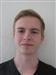
\includegraphics{pictures/s123161.png}%

\includegraphics{pictures/s123369.png}%
\end{figure}
22nd of May 2013

\thispagestyle{empty}
\newpage

 


\begin{abstract}
In this report we present the design and implementation of an arkanoid clone
called Smashing Bricks, that runs on an eZ8 microcontroller, displays graphics
in a terminal on a PC by transmitting ANSI codes over a UART, and plays sound
effects and a backing track generated by a Stellaris Launchpad microcontroller
that receives commands from the eZ8 over an SPI connection. The game also
includes ASCII art backgrounds generated from raster images and runs at
30 frames per second in a terminal. We show what
design considerations were made and how they were implemented in broad terms,
using flow charts and block diagrams to show control flow and connections
between modules.
We do not present a line by line walkthrough of the written code as
it is included in the appendix. The final design is a modular and easily
extensible design that contains three independent abstraction layers for
both the eZ8 and \emph{Stellaris Launchpad}. In the end we present screenshots
and a description of the gameplay.

\end{abstract}

\renewcommand{\abstractname}{resumé}
\begin{abstract}
Denne rapport gennemgår design og implementering af en arkanoid klon kaldet
Smashing Bricks, der kører på en eZ8 mikrocontroller. Spillets grafik vises i
en terminal på en PC der modtager ANSI koder fra microntrolleren over en UART.
Spillet inkluderer også baggrundsmusik og lydeffekter, der afspilles af en 
Stellaris Launchpad der modtager kommandoer fra eZ8 mikrocontrolleren over
en SPI forbindelse. Spillet har baggrundsbilleder i ASCII art der er genererede
fra raster billeder og det kører ved 30 frames per sekund i terminalen.
Vi viser hvilke design beslutninger der er taget og præsenterer en forklaring
af hvordan det er implementeret ved brug af flow charts der viser modulers
kontrol flow og blok diagrammer der viser deres indbyrdes forbindelser, men
 vi gennemgår ikke hver linje af koden da denne er tilgængelig i appendex.
Det endelige design indeholder tre uafhængige abstraktionslag for både
eZ8 og Stellarisen,  og det er modulært og let at udvide. Til sidst præsenterer
vi resultatet med screenshots og en beskrivelse af gameplayet.
\end{abstract}

%TODO whodunnit
\clearpage
\tableofcontents

\section{Introduction}
The aim of this report is to present the design process of an arkanoid game clone running
on an eZ8 microcontroller and displaying graphics in a terminal on a PC. The point in
making this game is to showcase good design practices when working with a medium sized
programming problem. This includes up front design with flow charts describing individual
program functionality, sensible project structuring and managing, three layered design
with layers that are independent of each other as well as documentation skills. \\

The report is structured in two main parts since we have used two different pieces of hardware,
The eZ8 microcontroller development board and a Texas Instruments Stellaris Launchpad. The
launcpad is used for sound playback and recieves control commands from the eZ8 over SPI.
Because the Stellaris Launchpad is a different piece of hardware it needs its own 
hardware abstraction layer, and as it provides a different functionality, the sound 
generation also has its own API. Therefore the report is split into a parts detailing
the design process of both the software running on the eZ8 and Stellaris Launchpad. \\


\section{Specification}
We have chosen to make an arkanoid like game with the following extensions

\begin{enumerate}
\item Continuously calculated reflection angle from the striker.
\item Bricks with any number of lives, colored after this number.
\item Background music.
\item Sound effects.
\item ASCII art backgrounds generated from real pictures.
\item Analog joystick input.
\item A score system.
\item Multiple levels.
\item Limited number of player lives.
\item 30 frames per second graphics.
\item Powerups.
\item Highscores saveable on permanent media.
\end{enumerate}

The list is ordered with items in descending priority. The last 2 items on the list
did not make it into the final game due to time constraints.

\section{Analysis}
As the game must be made to run on an eZ8 microcontroller, with limited performance capabilities, and display graphics in a terminal
 via ANSI commands sent over a relatively low bandwidth UART connection, performance must be taken into consideration and bottlenecks identified. \\

Generating the sound needed for background music and sound effects is a performance heavy task that we deemed
impossible to implement purely on the eZ8 microcontroller.
Therefore, the sound generation is offloaded to a Stellaris Launchpad microcontroller. 
This will then recieve commands from the eZ8 using SPI, such that the game running on the eZ8 can control
what sounds are being generated by the stellaris.\\

Displaying background images requires a lot of ANSI escape codes to be sent over the UART communication with
the terminal used for graphics. This is due to complex graphics having many different colors. As the UART on the eZ8 
development board is only capable of sending data at 115200Baud, this issue must be taken into account
in the software responsible for graphics if a new picture is to be rendered 30 times a second. \\

To make use of a joystick for controlling the striker it will also be necessary to use the ADC on the eZ8 development
board. 






\section{Design}
This section covers both game design and software architecture design, as well as the
design of the individual software modules.

\subsection{Game Design}
The game is an arkanoid clone and as such it is very simple and follows the general arkanoid formula of destroying
bricks using a ball that bounces around the screen. The ball will reflect itself off of a brick, wall
in the top of the playing space as well as two walls bordering the sides of the playing space.
There is nothing stopping at the bottom of the playing space, except the player controlled striker.
It is the players objective to control the striker such that the ball is reflected off of it and
hits all the bricks. Thereby destroying the bricks. \\

In this version of arkanoid, which we will henceforth refer to as Smashing Bricks, the player
upon starting a game is presented with a splash screen, followed by the first level. The levels
themselves contain a brick layout that can be changed as well as a monochrome background image.
Upon completion of the level, the full-color background image is revealed and the player can
move on to the next level. Once the player reaches the end of the game, the players score
will be presented and the option to restart the game will be available. \\

The score is incremented by a set amount every time a brick is hit or destroyed. If the player
misses the ball, another amount is subtracted from the score. If the players score goes below
0, the game is over and the player will have the option to restart the game. \\

The balls reflection from the striker is not actually a reflection, instead the direction
of the ball is changed according to where it hit the striker. As with all games, these
mechanics are based on their feeling and this to us felt like the most natural way to play.
Similarly the speed of the ball and striker are also based on feel. \\

Background music will play and sound effects are triggered every time the ball is reflected
from a brick, a wall or the striker. \\

The game only has a single difficulty, hard, this is due to the fact that we deemed slow and/or
easy arkanoid games to get boring too quickly. The game is therefore deliberately designed to 
force the player to quickly be able to estimate where the ball will reach the bottom again, as 
soon as it leaves the striker.

\subsection{Software Architecture Design}
Considerable time and effort went into insuring that the software itself would be modular and easily extensible.
As mandated, the software contains three layers. A hardware layer that is concerned only with
direct hardware manipulations, an API layer that is concerned with presenting general functionality to
the final application layer. The layers can be changed individually as long as they present the
same functionality to the layer directly above. \\

In our design, the hardware layer is relatively small as it only needs to deal with the following:

\begin{itemize}
	\item Handle ADC input for the joystick.
	\item Set up timers.
	\item Send data over SPI.
\end{itemize}

It is not necessary to write software that controls the UART as API functions covering  this
 is already provided by the default eZ8 libraries included in ZDS. \\

The API functions needed for general game applications are then the following.

\begin{itemize}
	\item Graphics.
	\item Sound.
	\item Math. (Sine, Cosine, fix point etc.)
	\item Input handling.
\end{itemize}

The API layer presents a general framework that can be used for any game application. If extra
functionality is needed it is also easily extensible. \\

To make the game application itself as modular and extensible as possible, we have utilized a
style of C programming that approaches object oriented programming as this is especially well
suited for games. To understand why, we must look at the general game application control flow. \\

Modern games run either with a fixed or a free running framerate, we will only discuss the fixed
framerate type as this is easier to work with for this application. Within every frame period, the
game situation is updated. This means getting input from the user and  updating the position of every object
, checking collisions and reacting accordingly etc. When this is done, the new situation is presented to the
 user by updating the graphics medium, in this case a terminal. The cycle then repeats until the game
ends. This can be split into 3 distinct operations that need to be performed within the main game loop:
Get input, update, render. This will be done at the standard 30 frames per second \\

The advantage of object oriented programming is that all game entities can then contain their own
update and render functions, eliminating the need to change exisiting code when a new game entity is added.
This also helps to avoid spaghetti code and deep nesting problems. While we are aware that object oriented
programming usually comes with significant performance overhead and as such is not suitable for a microprocessor,
we deem this to not be a problem as we do not a use truly object oriented style, only an approximate one, where every
entity is represented as a struct with function pointers to its inner "methods" and primitives for fields.
Only a small amount of glue code is needed to control the transition between levels and manage the game state. \\

Communication between modules follows the mantra that less is good. As such, the amount of information and functions
present to each other is kept at a minimum. This is done to keep the number of entry points to a module as small
as possible, thus making it possible to change the inner workings of a module without breaking external dependencies.
As functions and variables in C are confined to their own scope, the file in which they are declared, and this
scope can only be extended by including them in a header file, our header files are kept as simple as possible. \\

A block diagram of the modules and their communication paths can be seen in figure \ref{architecture_block}. In the
diagram, arrows represent in which direction function calls and commands travel, which typically means information
flows in the opposite direction. \\

\begin{figure}
	\center
	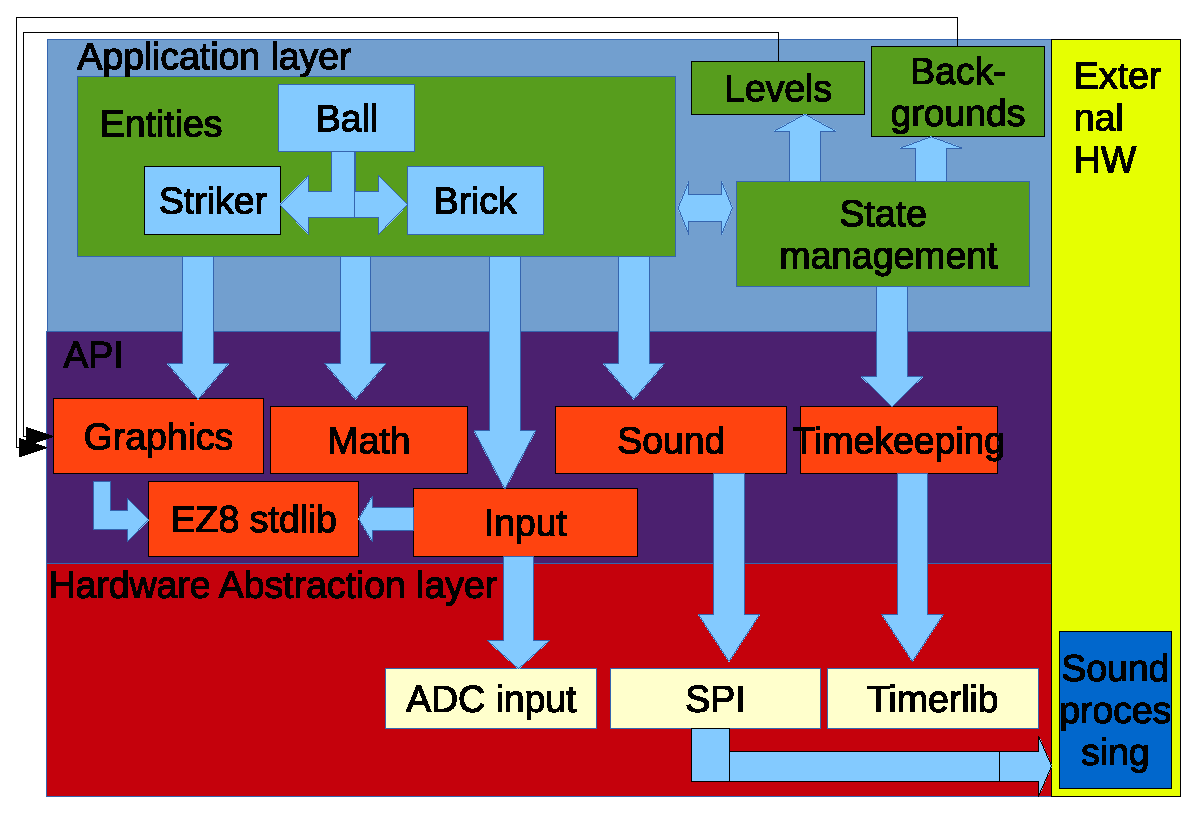
\includegraphics[scale=0.7]{pictures/architecture_block.eps}
	\caption{Block diagram of the software modules and their communication}
	\label{architecture_block}
\end{figure}

A flowchart depicting the top level control flow can be seen in figure \ref{top_flow}.

\begin{figure}
	\center
	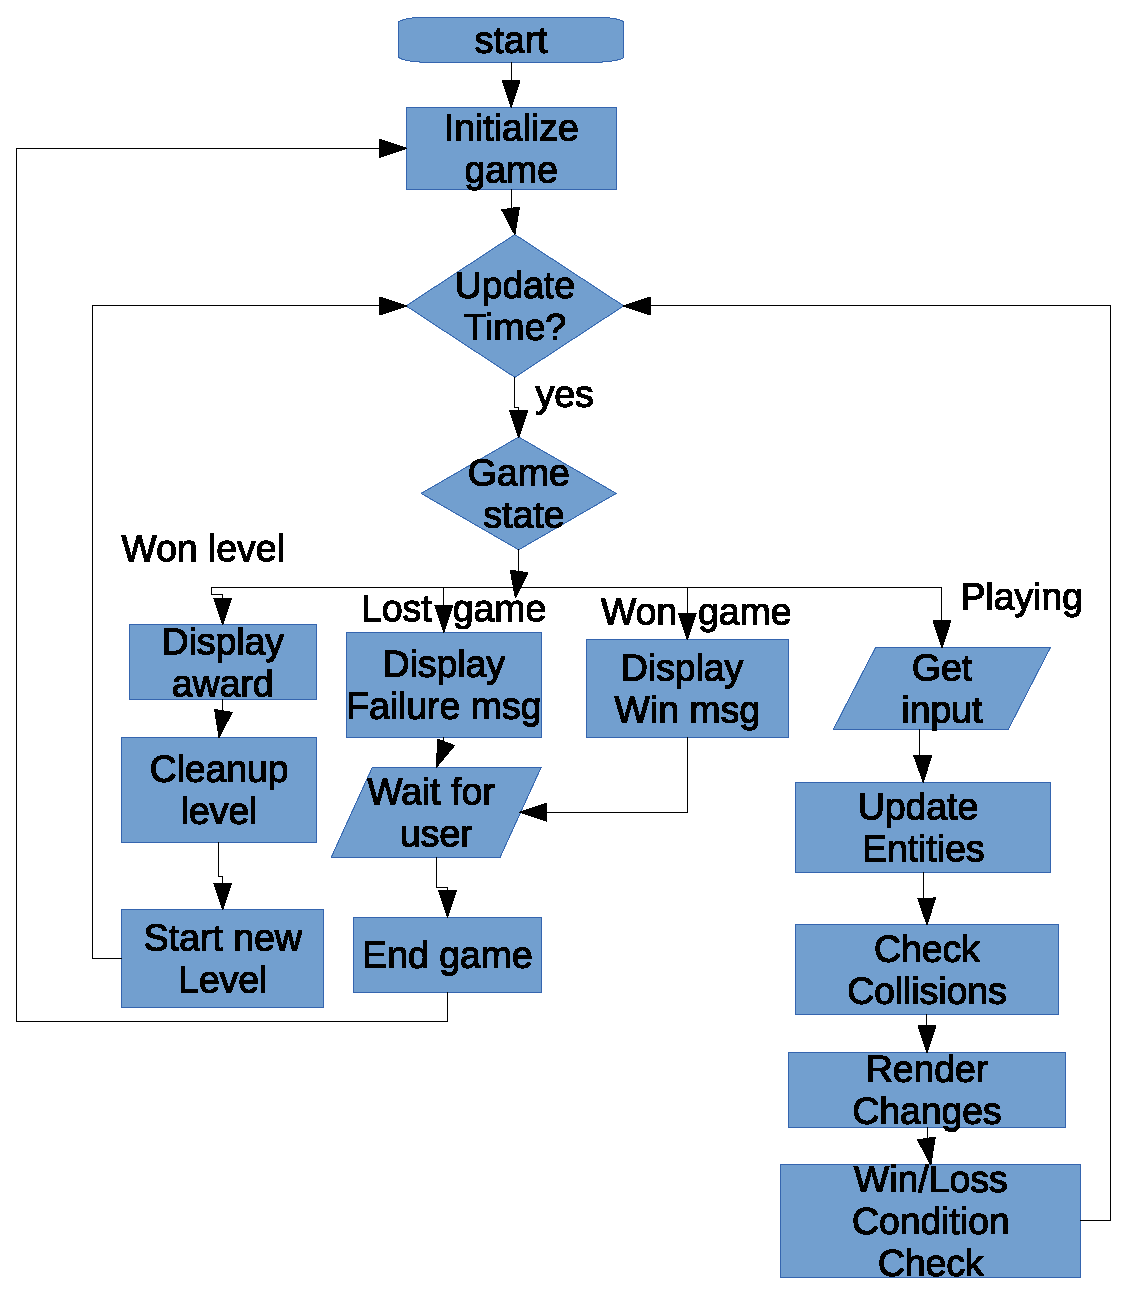
\includegraphics[scale=0.7]{pictures/top_flow.eps}
	\caption{Control flow at the top level}
	\label{top_flow}
\end{figure}


%% Gaming units

	\section{Implementation of Game Software}

This section deals with the implementation of the modules discussed in the design section.
Since it is pointless to describe exactly how the code performs its function, as this 
can be read directly from the code, it is described what the code does in  broad terms and why. 

\subsection{Hardware Abstraction Layer Implementation}
As mentioned before, the hardware layer is fairly thin as only three modules are needed for our game.

\paragraph{SPI module}
The setup\_SPI\_master() function  configures the hardware SPI module the eZ8 development board to run at max speed as a master.
The write\_spi() pulls the slave pin low, signaling the start of a transmission and places its argument in the SPI data register
which immediatly starts transferring the data. It then waits until the transmission is complete and returns.
The source is found in spi.c/h.

\paragraph{Timerlib}
The set\_timer() functions takes arguments to configure what timer to enable, what period the timer
should be set to, the priority, and what function should be called when the interrupt occurs. Currently
only one timer can be enabled and the timer select argument is simply ignored, so is the priority. 
The function calculates the needed reload values for the timer and enables TIMER0. The interrupt vector
is set to call a function which immediately calls the function passed as an argument using a function pointer.
The source is found in timerlib.c/h.

\paragraph{ADC input}
the ADC module is fairly simple. The setup\_joystick() function takes
no arguments and configures the PB0 pin on the eZ8 development board for its alternate ADC function.
The read\_joystick() function simply returns the most significant 8 bits of the current ADC sample.
The source is found in joystick.c/h.

\subsection{API Layer Implementation}
The API layer uses the functions provided by the hardware abstraction layer to present additional functionality to the application
layer.

\paragraph{Input Module}
The input module manages and presents a global array to the application layer. This global array contains the state of all inputs
and it is updated every time get\_input() is called. The array indexing is managed with an enumeration, such that
additions to the array do not destroy existing dependencies. The array is global because almost every module in the
application layer needs access to the current keystate or joystick value. The input array is only updated by the 
input module. Before being able to utilize joystick input, an application must first call setup\_input() which 
makes sure that the joystick ADC pins are enabled. The source is found in input.c/h.

\paragraph{Sound Module}
The sound module contains different named sounds that can be played by calling the play\_sound() function.
To be able to play sound, the SPI module must first be setup and so the sound module includes a
function for enabling the sound. The source is found in sound.c/h.

\paragraph{Math module}
The math module contains a macro for the cosine function and 8.8 fixed point math. Its only real
function is the sin() function. This takes an argument in 512-degrees and returns the
sine value of the angle from a lookup-table that was generated by an excel macro given in
the first weeks exercises. The source is found in math.c/h.

\paragraph{Timekeeping Module}
The timekeeping module simple calls through to the hardware layer to set up a timer. The source is found in
timekeeping.c/h

\paragraph{Graphics Module}
The graphics module utilizes the UART on the eZ8 board to send ANSI escape codes to a terminal on a PC.
The gotoxy(), clrscr() and color change functions simply send an ANSI escape code using printf() from 
the eZ8 stdlib. The set\_monochrome() and set\_background() functions manage a set of variables
that are global to the graphics.c file scope and not to the entire program. These are used by
the background drawing functions that calculate what color to place behind characters being drawn.
Changing the color for every character is extremely bandwith intensive, and therefore the current
color is kept track of by another set of locally global variables such that color change messages
only need to be sent when actually necessary. When the monochrome variable is set to true, all
images are drawn in black and white only. The source is found in graphics.c/h  

\subsection{Application Layer Implementation}
The application layer exclusively uses API functions to perform the game simulation and updating.

\paragraph{Main function}
The main function initialises the inputs, outputs, and the timer needed for the application. After this
it uses helper functions to start the game. Every time the timer fires an interrupt, a global update flag
is set to true which triggers updating and rendering of all entities as shown in figure \ref{top_flow}.
The main function acts as the state manager in the block diagram shown in figure \ref{architecture_block}

\paragraph{Levels Module}
The levels module contains all the game levels. These are represented as a struct that contains
information about how many bricks the level contains, which is needed for the bricks array
that holds all the bricks that need to be updated. The struct also contains the brick layout
for generating the brick entities in the right positions and a pointer to a background pointer, 
which is used for the load\_level() and end\_level() helper functions that display the background
image. The levels module holds a global variable used at the top level, the current level. The source
is found in levels.c/h.

\paragraph{Backgrounds module}
The backgrounds module contains constant arrays of generated ASCII art data. These arrays are used
to display the level backgrounds and are generated using a java program that transform a raster
art picture to ASCII art. The module also contains pointers to these constant arrays. Every
background takes up 8KB of space and is therefore saved in the ROM by enabling the compiler
directive that places all constant variables in ROM. Source is found in backgrounds.c/h.

\paragraph{Entities}
All entities use the same basic blueprint. A struct containing the variables that they can share
with other entities, position fields always in 8.8 fixed point format, function pointers
 to their specific render, update and collided functions, and
a void pointer to a struct containing encapsulated data that is only used by the entity itself. 
Using the void pointer makes it harder for other entities to use the data encapsulated in the
struct pointed to by the void pointer, which helps to avoid interdependencies. Every entity also
has a create and destroy function which makes it possible to allocate memory for the entity
and free it upon destruction. This needs to be done to avoid the entities going out of scope
and their data being overwritten. The function pointers to update, render and collided functions
makes the code at the top level clearer and easier to extend since the internal functions that
are pointed to can be changed at will without changing other code.

\paragraph{Ball Entity}
As the ball is the only entity that can collide with other entities, this entity provides its own 
collision detection, other entities simply employ boundary checks. The collision checking code
uses and ID passed to it to determine which entity the ball is currently checking against.
This allows the ball to act uniquely depending on which entity it collides with.
 The ball also holds the score
as it is convenient to represent the player as the ball instead of the striker. The ball
uses a polar representing of its velocity and angle such that it can move in any direction
and reflection calculations are easy to perform. A flowchart of the
 code called when a collision has been detected can be seen in figure \ref{ball_flow}.
Source is found in ball.c/h.

\begin{figure}
	\center
	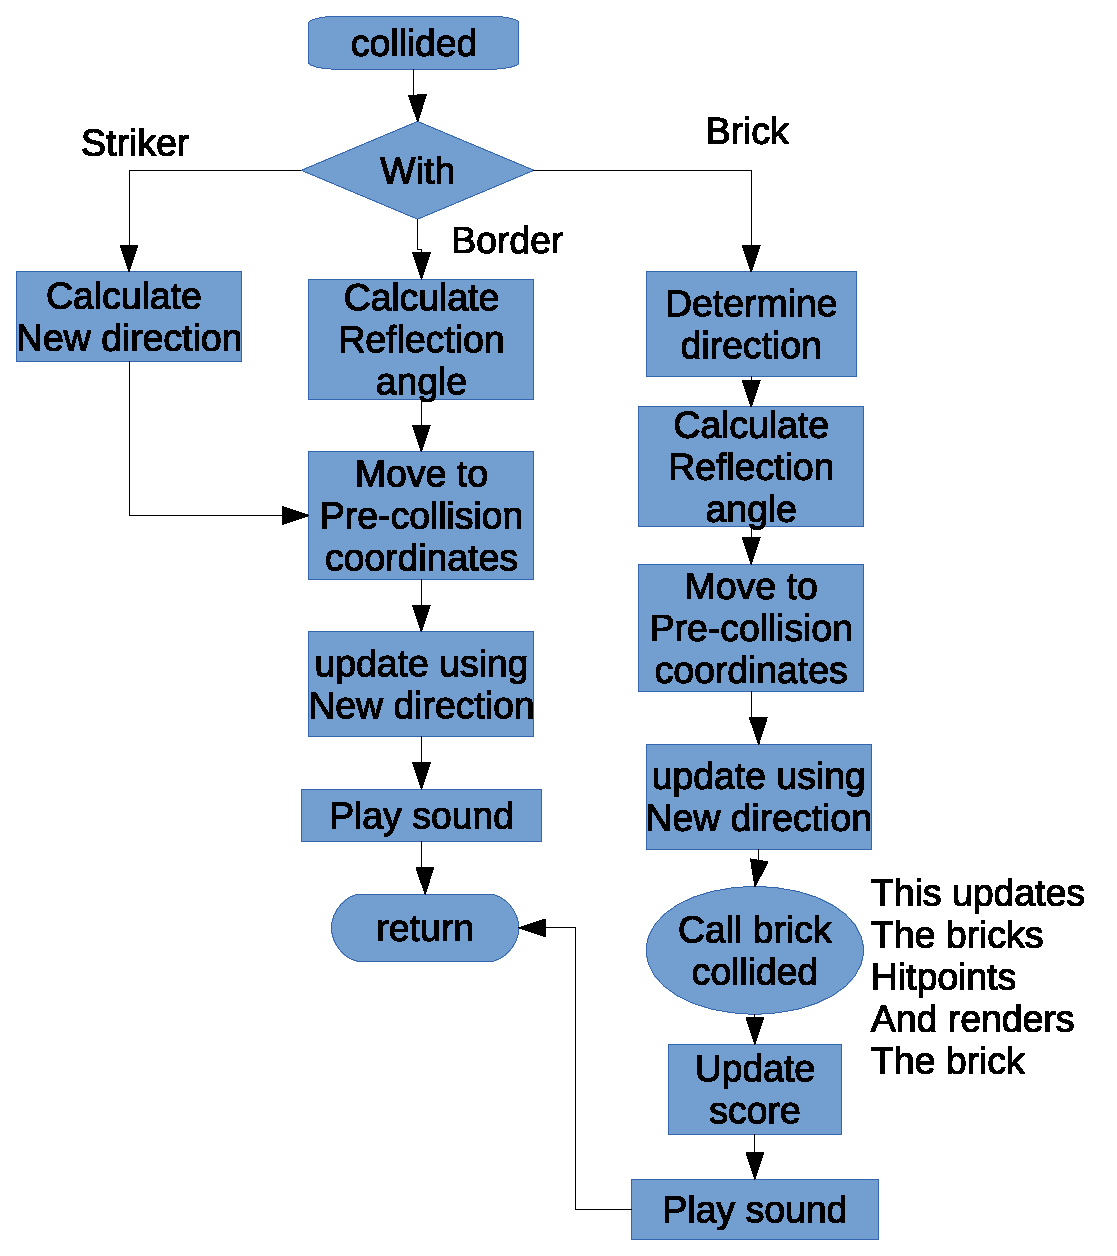
\includegraphics[scale=0.5]{pictures/ball_flow.eps}
	\caption{Program flow upon a ball collision, the redundancy in calculating the reflected
	direction when colliding with a brick is due to it being different depending on the direction
	from which the ball approached the brick.}
	\label{ball_flow}
\end{figure}

\paragraph{Striker Entity}
The striker entity polls the keystate/joystick value when updating its position. It then 
calculates a new position depending on the striker speed. When rendering, only the needed
characters are drawn instead of erasing the striker before drawing it, to maximize drawing
performance. The striker speed and reactivity to the joystick is based on testing for
what felt best. Source is found in striker.c/h.

\paragraph{Brick Entity}
The brick entity is only updated and rendered upon a collision since it cannot move. It is
drawn in a color determined by its current amount of hitpoints. Source is found in brick.c/h.

	\subsection{Game Testing}
Game testing was mostly done manually, by visual inspection of the game behaviour and
aid from the debugger. The game code was slightly modified to force edges cases to
occur so that time would not be wasted on waiting for them to happen naturally.
 This is of course not the most optimal way to test software,
however, for a game it is necessary. While unit and integration tests would have been helpful, and
would most definitely be included if we were to redo the project, manual game
testing would still need to be performed. The game testing also served a 
secondary purpose, besides verifying that the software was working as intended.
It allowed us to tweak the gameplay based on how good the game felt to actually play. \\

The SPI module was tested and debugged using a logic analyzer program for the stellaris 
launchpad.



% %Audio unit
\section{The audio module}
%baad stlye i know..
As the audio module is a somewhat independent module, the analysis and design
of the module has a section of its own.
 	\subsection{Audio module introduction}
The audio module will be run as an external application on a \emph{Texas
Instruments} \emph{Stellaris Launchpad}, communicating with the \emph{eZ8} via
\emph{SPI}.

The audio module performs the following:
\begin{itemize}
  \item Play and stop one song: \emph{Popcorn}
  \item The song has 3 voices
  \begin{itemize}
    \item Lead
    \item Bass
    \item Percussion
  \end{itemize}
  \item The module connects to the \emph{eZ8} with SPI and receives data as
  \emph{MIDI} messages.
  \item The module can play game specific sounds (bleeps when the ball hits
  anything and similar)
\end{itemize}

Since this section assumes some known knowledge about synthesizers, a small
introduction to subtractive synthesis is given in the next section.

\subsubsection{An introduction to subtractive synthesis}\label{synthxp}
Subtractive synthesis is one of the very popular methods of creating musical
notes. A very basic synthesizer is described in figure:~\ref{fig:basicsynth}

\stdfig{0.8}{audiomodule/basicsynth}{Block diagram of a basic
subtractive synthesizer, with examples of signal waveforms. A
sequencer is used as the source of notes. Note that the timing
of the sequencer signal examples is not one scale with the
rest of the signal examples.}{fig:basicsynth}

A steady stream of pulses enters the sequence and makes it advance through it's
pattern, here with a pattern length of 5. The sequencer output is used as the
input of the oscillator to control the frequency of it - this could just as well
be from a keyboard - The oscillator generates a harmonic rich output that is fed
into a resonant filter (2 pole low-pass here) to \emph{subtract} harmonics; then
the filtered signal is fed through an amplifier.

The cutoff frequency of the filter is controlled by the \emph{ADSR}, an acronym
for \emph{Attack Decay Sustain Release} this works as following:
\begin{itemize}
  \item Attack: After a trigger the output rises from 0
to max at a specified rate.
  \item Decay: The signal then falls to the sustain level at a specified rate.
  \item Sustain: As long ad the gate is high, the output is helt at the sustain
  level.
  \item Release: Once the gate is low, the output falls back to 0 at a specified
  rate.
\end{itemize}

The amplitude of the amplifier is controlled by an \emph{AHDSR}, the same as the
\emph{ADSR}, except a short delay, where the output is held at max - the hold
phase - is put in between the attack and decay stages.
 
	%analysis 
	\subsection{Audio module analysis}
The audio generation is very processor heavy - if more than monophonic
bleeps are desired that is. - To produce alias free audio in the full audible
range, the output has to be updated more than 40000 times a second.
Therefore this task is moved from the \emph{eZ8} to a \emph{Texas
Instruments} \emph{Stellaris Launchpad}, an evaluation-board for the 80MHz
\emph{ARM Cortex-4M} \emph{LM4F120H5QR} chip.
%TODO tilf�j link til http://www.ti.com/tool/EK-LM4F120XL

The \emph{LM4F120H5QR} is ideal as:
\begin{itemize}
  \item It has 64kB of FLASH memory, enough for a medium-size program and small
  wave-files;
  \item 32 bit processor, providing a solid frame for fast and
  precise generative sound synthesis;
  \item build in PWM module that width some external filtering can be used a a
  digital to analog converter, removing the need for an external ADC. Furthermore
  the output is powerful enough to drive small headphones at low volumes.
  \item We have past experience with the processor and associated tools, thus
  the time cost can be reduced by choosing this solution over another.
  
\end{itemize}

As the audio module has to play both a piece of music and sound-effects; a mix
of generated sounds and playback of wave-files is chosen.

The use of generated music cuts down the space a huge wave-file would take. 10s
of 8bit data at 44kHz is 0.44MB, we can't fit that in the 64kB FLASH of the
\emph{LM4F120}. On the other hand even at 80MHz speech synthesis becomes
troublesome, but if speech is re-sampled to ~10kHz it is still possible to make
out words. Percussion sounds can also be put in down-sampled wave-files, as
aliasing artifacts aren't a huge sacrifice when dealing with short, rhythmic
outbursts.



	%desing
	\subsection{Audio module design}

As described under the analysis, the audio module has to be capable of both
generating sounds and playing predefined wave-files. The processor is chosen to
run in real-time with a frequency of 44kHz, this is done to reduce aliasing
artifacts - in theory this is enough to allow an output spanning the full
audible range, given sufficient filtering and taking care not to generating any
tones above the nyquist-frequency; we did however not have the time to dive
fully into this theory and thus some aliasing will occur.

The design of the audio module will be done like a digital model of a modular
synthesizer, taking inspiration from eg. the free-to-try software
\emph{SynthEdit0} in which different block (oscillators, filters, transient
generators, wave-file players etc.) can be connected to form whole synthesizers.
See figure:~\ref{fig:synthedit}.

\stdfig{0.8}{audiomodule/synthedit.jpg}{The design of the synthesizers took
inspiration from the block approach as seen in eg. the free program
\emph{Synth Edit} \cite{SynthEdit}. Image from \cite{SEimg}}{fig:synthedit}

This approach allows for both easy programming of the modules, as this becomes
an highly manageable problem; easy programming of the synthesizers, this is just
connecting the blocks; and provides an easily expandable and reusable library.
This also allows for easy programming reusable container modules, eg. a
standard synthesizer.

Communication is done over SPI, using MIDI (\emph{Musical Instrument Digital
Interface}) commands. This allows for a MIDI interpreter module, working in
similar ways as all other modules.

\subsubsection{Overview}
We decided that the background music should be the 80'es classic
\emph{Popcorn}.
For this we need three voices, lead, bass and percussion.
The score is stored in 6 arrays (notes and gate/trigger for each voice) and a
sequencer goes through this array, giving notes and triggers to the synthesisers
and wave-player. This is illustrated in figure:~\ref{fig:audioflow}

\stdfig{0.8}{audiomodule/audioflow}{Block diagram of the audio
module}{fig:audioflow}

The two red blocks, \emph{raw Synth} and \emph{filter Synth} are the
synthesisers for the lead voice and the bass voice respectively. These modules
are application specific.

For the lead voice we create a module called `\emph{RawSynth}, because this only
contains the bare minimums for a synth: An oscillator with a wave-shaper and a
\emph{AHDSR} module, controlling the volume. The wave shape is set to a stepped
saw-wave. See figure:~\ref{fig:rawsynth} for a block diagram.

\stdfig{0.8}{audiomodule/rawsynth}{Block diagram of the RawSynth used for the
lead voice}{fig:rawsynth}

For the bass voice we choose a synth with a 2-pole resonant state variable
filter, using the low-pass, doing a downward sweep for a synthy \emph{``dauww''}
sound. a block diagram for this can be seen in figure:~\ref{fig:filtersynth}.
This module we name \emph{FilterSynth}, a square wave is chosen for the
wave table, as this gives a nice tone for the bass (the fundamental is strong
in a square wave, compared to eg. saw wave)

\stdfig{0.8}{audiomodule/filtersynth}{Block diagram of the FilterSynth used for
the bass voice}{fig:filtersynth}

\subsubsection{Design of the core modules}
The following core modules were designed:
\begin{itemize}
  \item VCO: A basic oscillator with an input for the note to play and a saw
  wave output, no bandwidth limiting.
  \item LFO: A basic low frequency oscillator with a saw wave output and a
  \emph{tick} output, a delta function once every cycle.
  \item Sequencer: A sequencer, takes an array and turns it into a sequence -
  outputting each element in the array one at a time. The sequencer advances
  when the tick input is high and resets when the reset is high. The sequencer
  also has an output producing a delta function when looping around.
  \item LowPass: A simple 1-pole \emph{IIR} low-pass filter. Has an input for
  the signal and filter coefficient. This module was not used in the final product.
  \item SVF: A 2-pole resonant state variable filter. Has inputs for signal,
  filter coefficient, damping coefficient and outputs for hi-pass, band-pass and
  low-pass.
  \item AHDSR: \emph{Attack Hold Decay Sustain Release} module as described in
  section \ref{synthxp}. Has inputs for trigger, gate and the 5 parameters. only
  has one output.
  \item WaveShaper: A module capable of turning a saw wave from the VCO into any
  wave-shape - provided this wave-shape is given in an array. Can also perform
  bandwidth-limited wave-shaping if the supplied array supports it.
  \item MidiInterpreter: A module capable of reading from a FIFO (\emph{First
  In First Out}, as opposed to a stack) buffer and interpreting these signals.
  Has outputs for note: the last note played; trigger: high if the note was
  played in the current frame and playing: indicating if the music should be
  playing or not. Ideally there would be a ``note on'' and ``trigger'' array for
  every note (127 notes) on every midi channel (8 channels) - but this was not
  optimal for the given processor.
  \item OneShotter: A module for playing back small wave-files. It can
  re-trigger and takes a pointer to an array, storing the wave-file and the
  length of said file as arguments when updating.
\end{itemize}

\subsubsection{Design of the FIFO buffer}
A general utility structure \emph{FIFOBuffer} is designed, this module has the
following functions:
\begin{itemize}
  \item push: Pushes a data point into the beginning of the FIFO, returns 1 on
  success and 0 if the buffer is full.
  \item peak: Get the value of a data point a specified length from the end of
  the FIFO. Returns 0 if no data point exists here and 1 if it does.
  \item pop: Pop a data element from the end of the FIFO. Returns 1 if there
  was an element to pop and 0 if the FIFO is empty.
\end{itemize}

	%implementation
	\subsection{Audio module implementation}

The structure of the program deviates a bit from the three layers described in
\cite{Lect2} on slide 9, there is no application interface layer - as seen in
figure:~\ref{fig:overview}

\stdfig{0.8}{audiomodule/overview}{Block diagram of overall program
structure}{fig:overview}

The two main reasons for this is:
\begin{itemize}
  \item There are very few functions in this layer - a
layer more would just be a pass-through layer.
  \item For testing the application had to be ported to \emph{Windows}
\end{itemize}
	%result (wave files)
	\subsection{Testing the audio module}
As mentioned, the application was made so it could run smoothly on both the
\emph{Stellaris Launchpad} an on \emph{Windows}. Having the possibility to run
the application and saving a \emph{.WAV} file with the output was a huge
benefit, as the debugging tool only provided momentary debugging, but not the
possibility to view the output as a whole.
The testing could thus be performed as a mix of both listening and visual
inspection. A picture from the output wave-form can be seen in
figure~\ref{fig:wve}

\stdfig{0.8}{audiomodule/wve}{An excerpt of the output file, generated by
playing \emph{Popcorn}, at the beginning of the dark-gray area we see a
percussive sound (burst of noise) then we see the bass synth square-wave with
an applied resonant low-pass filter. The small ``jitters'' are the lead
voice}{fig:wve}

The only way to thoroughly test this system would be to make small test
applications, testing each module - this however would be a very slow process
and would take up a lot of space in the report. It was somewhat done
mid-project, when something didn't work as expected the application would be
rewritten to only feature the troubling module to isolate and remove the error
- but this was not documented in due time.

\subsection{Audio module results}
Without connection to the game, the audio module cannot do much - as it lacks
the message to start the music - and to play the sound effects.
This can - however - be bypassed, when using the debugging tool; we can change
the vale of registers to ``cheat'' the audio module into thinking, it has gotten
the required messages.

The Popcorn song can be herd in the included files: \emph{PopcornStellaris.WAV}
and \emph{PopcornWindows.WAV}.
They can also be found on the following webpages:\\
Sounds from the \emph{Stellaris Launchpad}:
\url{https://soundcloud.com/skrogh/popcorn-stellaris}\\
Sounds from \emph{Windows}: \url{https://soundcloud.com/skrogh/popcorn-windows}



	
	


%result?
	
\section{The resulting game}
The end result is a playable arkanoid game. Upon starting the game, the ASCII art title screen
shown in figure \ref{title} is displayed. After proceeding from the title screen, the first
level starts and the player can control the striker using a potmeter connecting to the eZ8
development board. In figure \ref{screenshots} a few screenshots from the game can be seen. \\

The game is very hard and unforgiving as you start with a score of zero and lose 25 points every
time you miss the ball. However the skill need to complete the game can quickly be
aquired. \\

The game runs at 30 frames per second without skipping frames, which makes for a very
smooth visual experience. The song "Popcorn" plays in the background, and every time
the ball hits a brick, a border or the striker, a sound is played.
 The dark backgrounds function well with the high contrast
color of the ball and striker. If the player dies, he/she is presented with a screen
encouraging them to retry the game, if the user accepts the game will automatically restart.
If the player manages to win the game, he/she is presented with a win message and the final
score, as well as the option to play again.  It is hard to describe the gameplay apart from the
provided screenshots. The reader is encouraged to refer to the gameplay manual and
try playing the game. It should be noted that the game can only be played in the PuTTY terminal
due to the resolution and color use.

\begin{figure}
	\center
	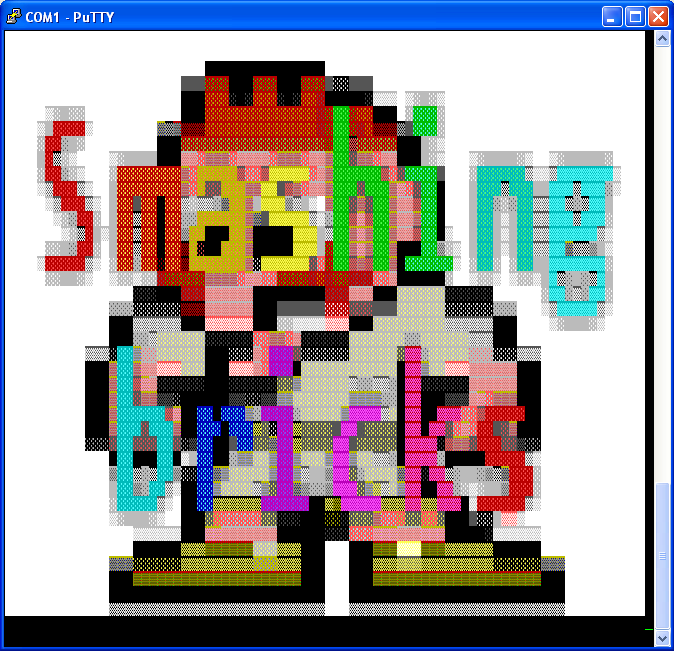
\includegraphics[scale=0.5]{pictures/title_screen.PNG}
	\caption{The Smashing Bricks title screen}
	\label{title}
\end{figure}

\begin{figure}
	\center
	\begin{subfigure}[t]{\columnwidth}
		\center
		\begin{subfigure}{0.3\linewidth}
			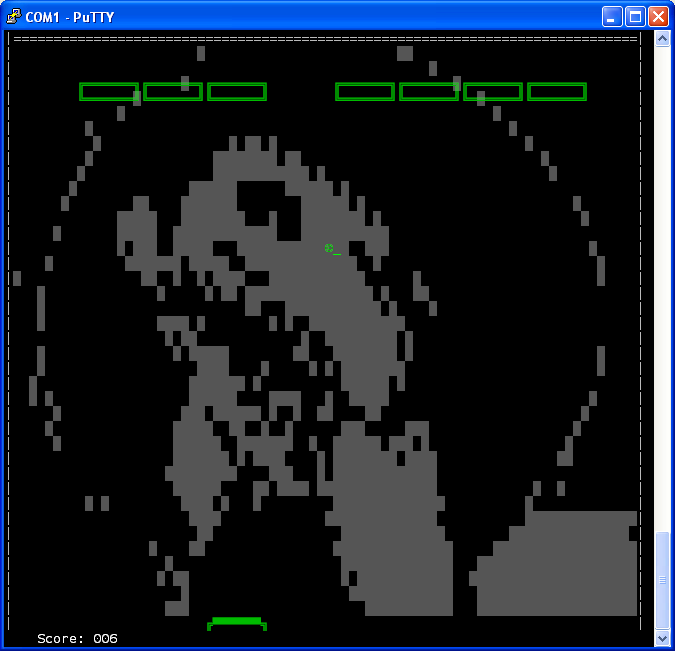
\includegraphics[scale=0.3]{pictures/level_1.PNG}
		\end{subfigure}
		\begin{subfigure}{0.3\linewidth}
			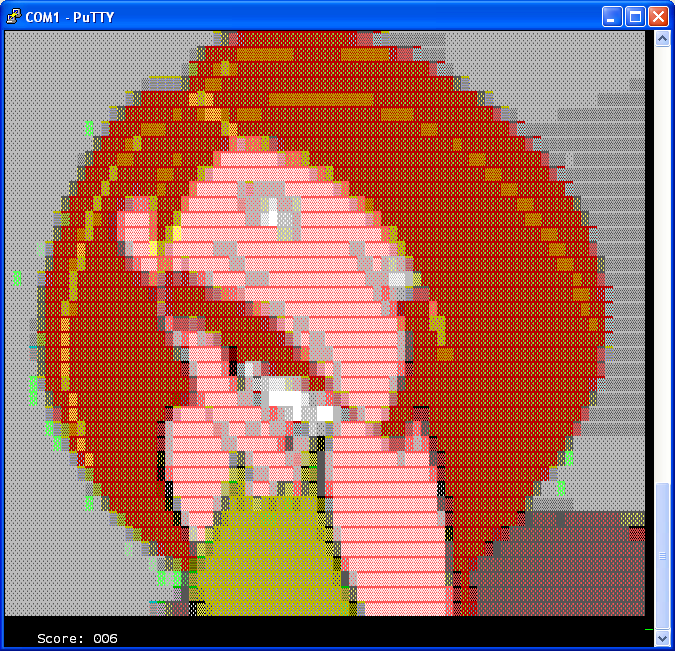
\includegraphics[scale=0.3]{pictures/level_1_complete.PNG}
		\end{subfigure}
		\begin{subfigure}{0.3\linewidth}
			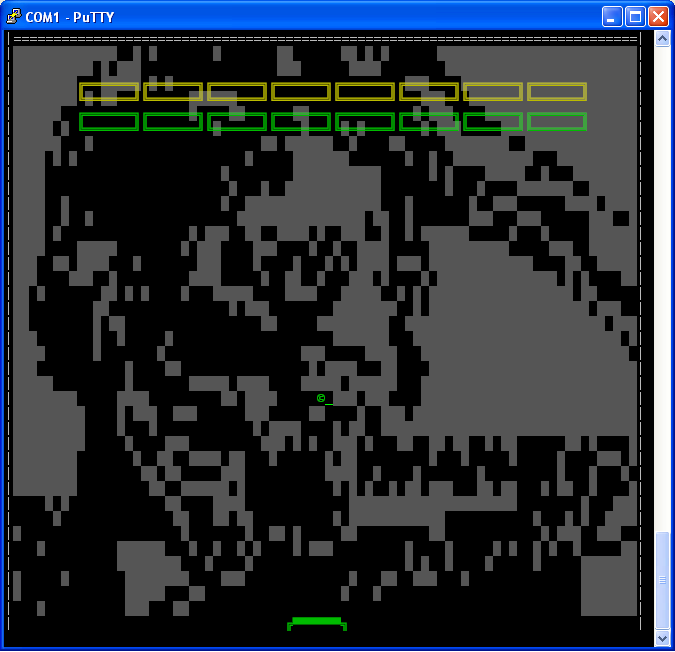
\includegraphics[scale=0.3]{pictures/level_2.PNG}
		\end{subfigure}
	\end{subfigure}
	\begin{subfigure}[c]{\columnwidth}
		\center
		\begin{subfigure}{0.3\linewidth}
			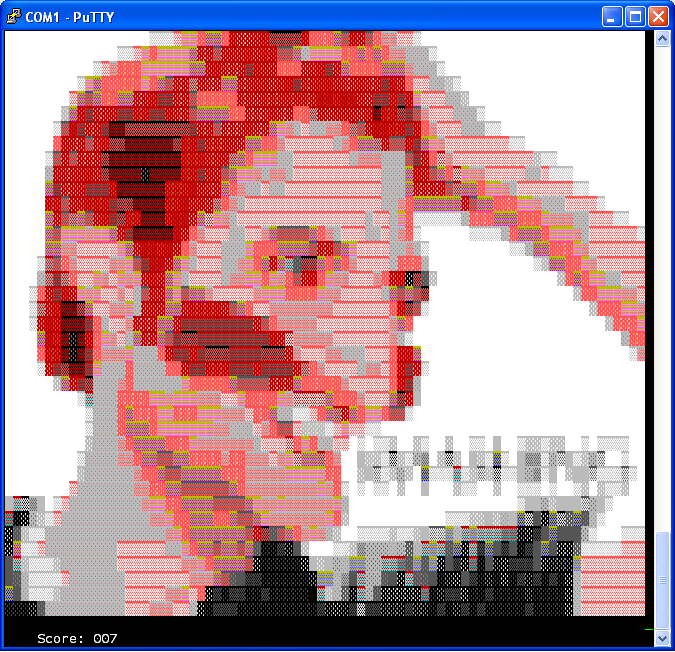
\includegraphics[scale=0.3]{pictures/level_2_complete.PNG}
		\end{subfigure}
		\begin{subfigure}{0.3\linewidth}
			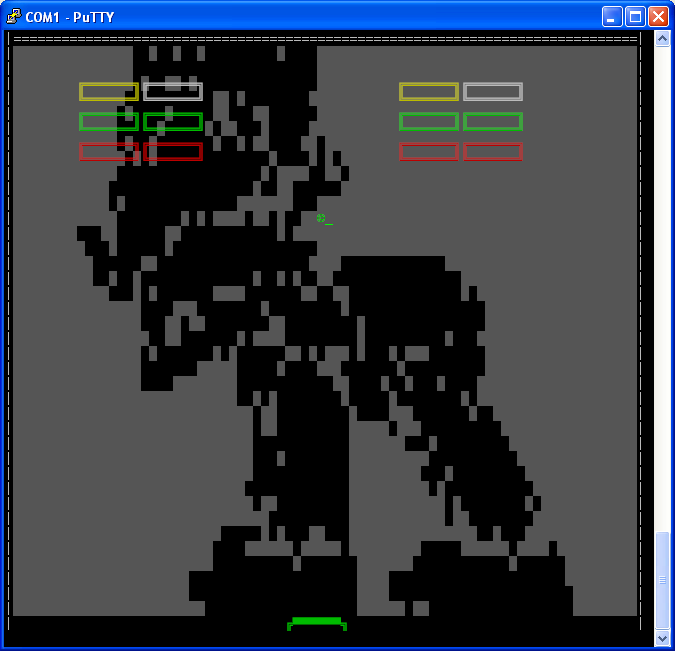
\includegraphics[scale=0.3]{pictures/level_3.PNG}
		\end{subfigure}
		\begin{subfigure}{0.3\linewidth}
			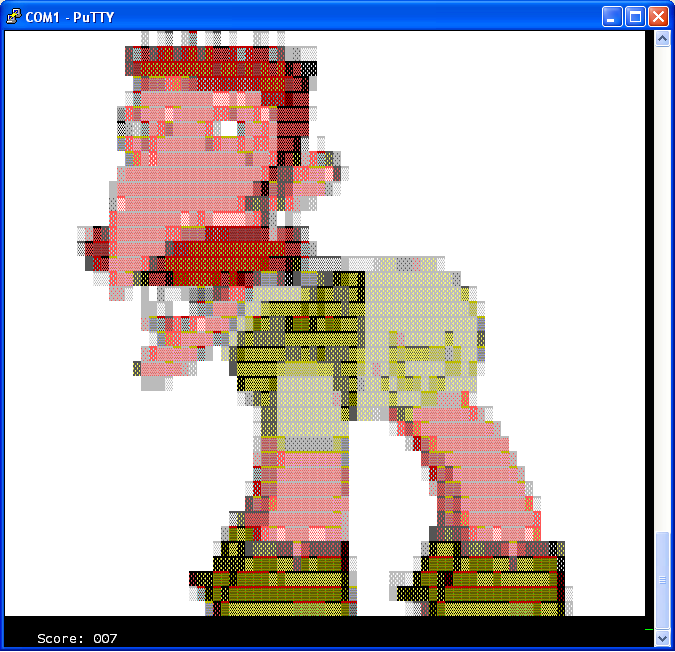
\includegraphics[scale=0.3]{pictures/level_3_complete.PNG}
		\end{subfigure}
	\end{subfigure}
	\begin{subfigure}[b]{\columnwidth}
		\center
		\begin{subfigure}{0.3\linewidth}
			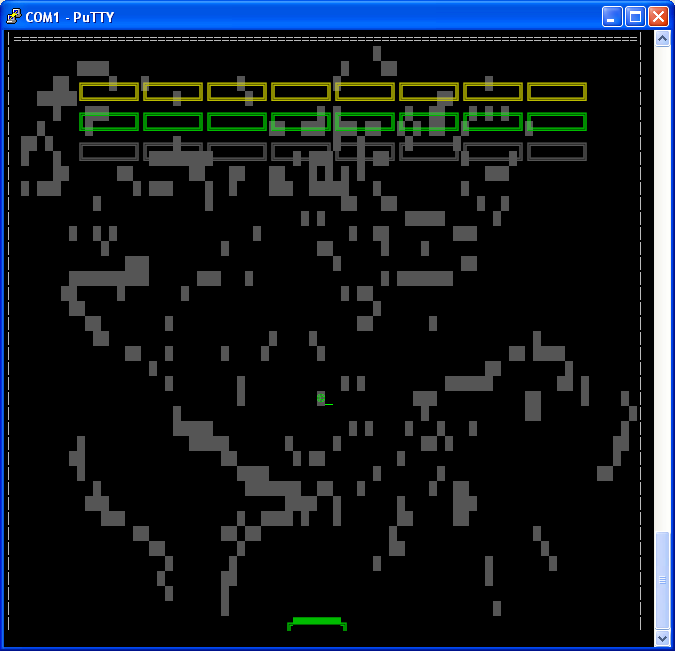
\includegraphics[scale=0.3]{pictures/level_4.PNG}
		\end{subfigure}
		\begin{subfigure}{0.3\linewidth}
			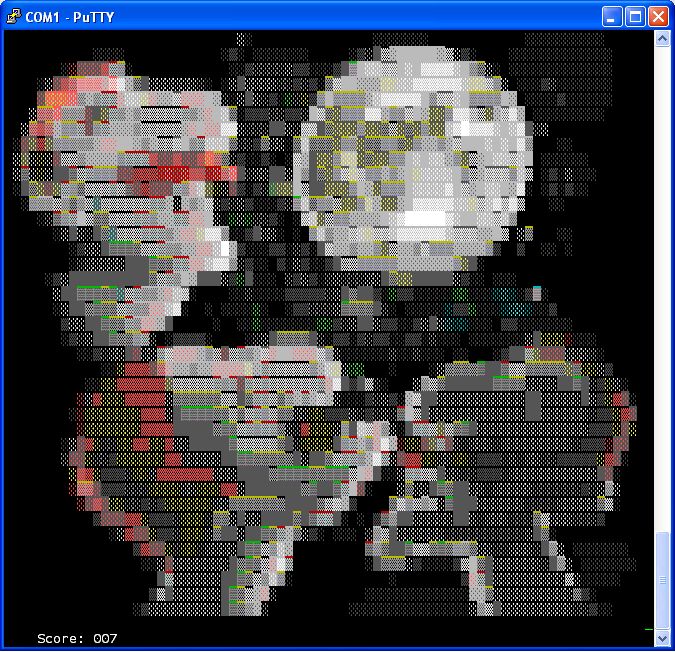
\includegraphics[scale=0.3]{pictures/level_4_complete.PNG}
		\end{subfigure}
		\begin{subfigure}{0.3\linewidth}
			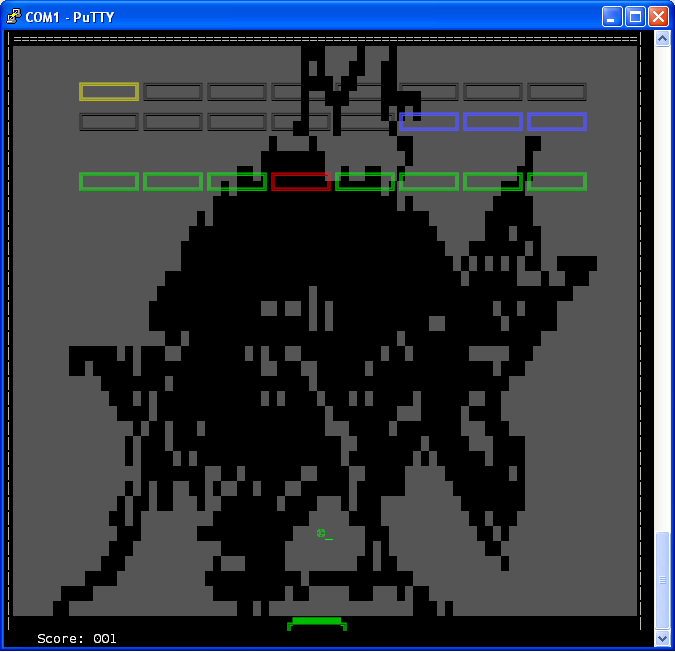
\includegraphics[scale=0.3]{pictures/level_5.PNG}
		\end{subfigure}
	\end{subfigure}
	\caption{Collection of screenshots from Smashing bricks}
	\label{screenshots}
\end{figure}

%discussion
	\Section{Discussion}


%conclution
	\section{Conclusion}
We have created an arkanoid clone, named Smashing Bricks, that runs on an eZ8 microcontroller
 development board and communicates with a Stellars Launchpad microcontroller to produce sound effects
that go along with the game. The software has been designed to be modular and
easily extensible. We believe we have succeeded in this, since modules are self contained, 
and provide a few well defined entry points for other modules to use. The final game has
the following features:
\begin{itemize}
	\item Continuously calculated reflection angle from the striker.
	\item Bricks with any number of lives, colored after this number.
	\item Background music.
	\item Sound effects.
	\item ASCII art backgrounds generated from real pictures.
	\item Analog joystick input.
	\item A score system.
	\item Multiple levels.
	\item Limited number of player lives.
\end{itemize}
Which is all but the two lowest priority items on our wanted feature list. The developed API and application code
would allow for these features being added with only minor changes to the existing code.


%litterature
\bibliographystyle{IEEEannot} %eller et andet setup?
\bibliography{audio_module/litt}
% build from cmd with 
%"C:\Program Files\pgm\MiKTeX 2.9\miktex\bin\x64\bibtex.exe" -include-directory="C:\Users\Soren\Git\30010\rapport\rapport" -include-directory="C:\Users\Soren\Git\30010\rapport\rapport\tmp" "C:\Users\Soren\Git\30010\rapport\rapport\tmp\main.aux"

%appendix
\appendix
\section{Manual}

\subsection{SMASHING BRICKS!}
Thank you for acquiring the \emph{Smashing Bricks} game,
Nigel Thornberry, not only known for his abeyance in the children's TV series
\emph{The Wild Thornberrys} but also the deep realms of the \emph{interwebs} for
his \emph{smashing} appearances in images all over the \emph{memeverse}
(\url{http://knowyourmeme.com/memes/nigel-thornberry-remixes}) wants to play a game with you.

Nigel is not hiding in Africa this time, but right in from of you! All you have
to do is uncover his manly face!

\subsubsection{Setting up the Nigel entertainment System}

\subsubsection{Setting up the display:}
Plug the \emph{Serial cable} of your \emph{Nigel Entertainment system (eZ8
board)} into the nearest data-machine, open your favourite terminal.

Use a display of at least 80x40 characters, without automatic line warp.
Make sure "Bolded text is a different colour" or similar is checked.
Set UART speed to 115200BAUD
For the best experience and the truest colors we recommend using the PuTTy terminal

\subsubsection{Setting up sliding input}
Plug the cable from the sliding potentiometer into the upper rightmost
pin-headers on the \emph{Nigel Entertainment system (eZ8
board)}

\subsubsection{Setting up the external audio noisemaker}
you will need the four supplied jumper cables for this task connect the pins
from the red \emph{Stellaris Launchpad} board on the left side in the table
with the purple \emph{eZ8} board on the right-side of the table:
\begin{align*}
GND &\leftrightarrow GND\\
PD0 &\leftrightarrow CLK\\
PD1 &\leftrightarrow SS\\
PD2 &\leftrightarrow MOSI
\end{align*}

Now connect the external filter so the black wire goes to $GND$ and the green to
$PF2$

Remember to power the device through the supplied \emph{USB} cable. If you don't
want foreign drivers from \emph{Texas} you can use the input labeled ``device''
and switch the power button to ``device''.

\subsection{You are now ready to play!}
\subsubsection{How to play}
Begin the game by pressing $S$ on the keyboard. A ball, a slider and some bricks
will appear. Move the slider with the sliding potentiometer (for a challenge
turn it upside down!) and catch the ball to throw it at the bricks. If you hit
the bricks enough, they will crumble and disappear.

\subsubsection{Loosing the game}
Hitting bricks will award you with points, 1 point for each hit, and 5 for
each brick you destroy. (Occasionally you may hit the corner off of a brick -
sorry no extra points for doing so). Should you drop the ball a penalty of -25
is put upon you - And the good Thornberry will laugh at you with his erring
voice. If your score drops bellow 0 you loose and must start over your hunt for
Sir Thornberry.

\subsubsection{Winning the game}
Should you clear all the brick in a level, the blurred background image will
reveal itself, Nigel will congratulate you in his sweet, British voice and you
will move on to a new, harder level.
Should you clear all the levels you will not only be congratulated, but also have seen a lot of Nigel
images - can you guess where all of them originate from?!







\section{Game module source code}

\subsection{Application layer}
\lstinputlisting{termanoid/src/applicationlayer/main.c}

\lstinputlisting{termanoid/include/applicationlayer/constants.h}

\lstinputlisting{termanoid/include/applicationlayer/striker.h}
\lstinputlisting{termanoid/src/applicationlayer/striker.c}

\lstinputlisting{termanoid/include/applicationlayer/levels.h}
\lstinputlisting{termanoid/src/applicationlayer/levels.c}

\lstinputlisting{termanoid/include/applicationlayer/brick.h}
\lstinputlisting{termanoid/src/applicationlayer/brick.c}

\lstinputlisting{termanoid/include/applicationlayer/ball.h}
\lstinputlisting{termanoid/src/applicationlayer/ball.c}

\lstinputlisting{termanoid/include/applicationlayer/backgrounds.h}

\lstinputlisting{termanoid/src/applicationlayer/backgrounds.c}

\subsection{API layer}

\lstinputlisting{termanoid/include/API/graphics.h}
\lstinputlisting{termanoid/src/API/graphics.c}

\lstinputlisting{termanoid/include/API/input.h}
\lstinputlisting{termanoid/src/API/input.c}

\lstinputlisting{termanoid/include/API/lut.h}
\lstinputlisting{termanoid/src/API/lut.c}

\lstinputlisting{termanoid/include/API/math.h}
\lstinputlisting{termanoid/src/API/math.c}

\lstinputlisting{termanoid/include/API/sound.h}
\lstinputlisting{termanoid/src/API/sound.c}

\lstinputlisting{termanoid/include/API/timekeeping.h}
\lstinputlisting{termanoid/src/API/timekeeping.c}

\subsection{Hardware interface layer}

\lstinputlisting{termanoid/include/HWapi/joystick.h}
\lstinputlisting{termanoid/src/HWlib/joystick.c}

\lstinputlisting{termanoid/include/HWapi/spi.h}
\lstinputlisting{termanoid/src/HWlib/spi.c}

\lstinputlisting{termanoid/include/HWapi/timerlib.h}
\lstinputlisting{termanoid/src/HWlib/timerlib.c}



\section{Audio module source code}

\subsection{Application}

\lstinputlisting{Synth_src/app/main.c}

\lstinputlisting{Synth_src/app/instruments.c}
\lstinputlisting{Synth_src/app/instruments.h}

\lstinputlisting{Synth_src/app/drums.h}
\lstinputlisting{Synth_src/app/nigel.h}
\lstinputlisting{Synth_src/app/popcorn.h}
\lstinputlisting{Synth_src/app/wavetables.h}

\subsection{FIFO}

\lstinputlisting{Synth_src/util/FIFO.h}
\lstinputlisting{Synth_src/util/FIFO.c}

\subsection{synth\_lib}

\lstinputlisting{Synth_src/synth_lib/generalModules.h}
\lstinputlisting{Synth_src/synth_lib/generalModules.c}

\lstinputlisting{Synth_src/synth_lib/MIDI.h}
\lstinputlisting{Synth_src/synth_lib/MIDI.c}

\lstinputlisting{Synth_src/synth_lib/oneShotter.h}
\lstinputlisting{Synth_src/synth_lib/oneShotter.c}

\lstinputlisting{Synth_src/synth_lib/waveshaper.h}
\lstinputlisting{Synth_src/synth_lib/waveshaper.c}

\subsection{Hardware, for \emph{Windows}}

\lstinputlisting{Synth_src/hardware_windows/hardInterface.h}
\lstinputlisting{Synth_src/hardware_windows/hardInterface.c}

\lstinputlisting{Synth_src/hardware_windows/make_wav.h}
\lstinputlisting{Synth_src/hardware_windows/make_wav.c}

\subsection{Hardware, for \emph{Stellaris Launchpad}}

\lstinputlisting{Synth_src/hardware_stellaris/hardInterface.h}
\lstinputlisting{Synth_src/hardware_stellaris/hardInterface.c}

\lstinputlisting{Synth_src/hardware_stellaris/lm4f120h5qr.cmd}
\lstinputlisting{Synth_src/hardware_stellaris/startup_ccs.c}
\section{Java utility tools}

\subsection{Tool for converting bitmaps to array of characters and
freground/background terminal colors}

\lstinputlisting[language=java]{Java_tools/tools/src/Imager.java}

\subsection{Tool for converting text file with score to array of sequencer data}

\lstinputlisting[language=java]{Java_tools/tools/src/Transcriber.java}

\subsection{Tool for converting 16bit signed \emph{.WAV} files to unsigned 8bit
arrays}

\lstinputlisting[language=java]{Java_tools/tools/src/WaveTest.java}
\lstinputlisting[language=java]{Java_tools/tools/src/WavFile.java}
\lstinputlisting[language=java]{Java_tools/tools/src/WavFileException.java}
\section{Journal}
\subsection{Exercise 1 and 2 }
\lstinputlisting[caption=exercise 2 main file]{"../../src/exercise2/main.c"}
\lstinputlisting[caption=exercise 2 ansi c file{"../../src/include/ansi.c"}
\lstinputlisting[caption=exercise 2 ansi h file]{"../../src/include/ansi.h"}

\subsection{Exercise 3 and 4 }
\lstinputlisting[caption=exercise 3/4 main file]{"../../src/exercise4/main.c"}
\lstinputlisting[caption=exercise 3/4 lut file]{"../../src/exercise4/lut.c"}
\lstinputlisting[caption= exercise 3/4 lut h file]{"../../src/include/luh.h"}

\subsection{Exercise 5 }
\lstinputlisting[caption=exercise 5 main file]{"../../src/exercise5/main.c"}

\subsection{Exercise 6 }
\lstinputlisting[caption=exercise 6 main file]{"../../src/exercise6/main.c"}

\subsection{Exercise 7 and 8 }
\lstinputlisting[caption=exercise 7/8 main file]{"../../src/exercise78/main.c"}
\lstinputlisting[caption=exercise 7/8 charset header file]{"../../src/include/charset.h"}
\lstinputlisting[caption= exercise 7/8 LED c file]{"../../src/include/LED.c"}
\lstinputlisting[caption= exercise 7/8 LED h file]{"../../src/include/LED.h"}




%TODO journal






\end{document}


